\documentclass[conference]{IEEEtran}
\usepackage[T1]{fontenc}
\usepackage{amsmath,amssymb}
\usepackage{graphicx}
\usepackage{booktabs}
\usepackage{cite}
\usepackage[hidelinks]{hyperref}
\usepackage{float}

% STRUCTURE ONLY: expand the sections in a later writing pass.
% Sources: ../../main.md, ../../report_angles.md, REPORT_PLAN.md,
% and evidence_register.csv. Comments below are writing instructions,
% not established findings. Leave unavailable results blank.
% Budget: six IEEE pages including references; contribution statement
% may occupy a separate seventh page. Recheck after the prose is written.
% Scope: one-ball behaviour cloning; further model optimisation is shelved.

\title{Learning to Catch with Behaviour Cloning:\\
Accuracy and Closed-Loop Failure Analysis}
\author{\IEEEauthorblockN{William Boyd, Nick Wright, Yiyan Wang}
\IEEEauthorblockA{University College London\\London, United Kingdom}}

\begin{document}
\maketitle

\begin{abstract}
% Write last: task, method, verified results, diagnostic contribution,
% and main limitation. Distinguish historical and reproduced results.
\end{abstract}

\begin{IEEEkeywords}
Imitation learning, mobile manipulation, robotic catching, evaluation
\end{IEEEkeywords}

\section{Introduction}
\subsection{Problem and Scope}
To catch a moving ball, a robot can move its hand to different points along the ball’s trajectory, changing the problem from reaching one fixed target to choosing between several valid positions. We extend the original fixed-target reaching task to moving target interception ("ball-catching"), still using the robot with the mobile base and seven-joint arm. Behaviour cloning is used to train a neural network to imitate the commands generated by the expert controller.

A model may closely match the expert’s recorded commands but still miss the ball when controlling the robot, because each small mistake changes the robot’s position and affects the movements that follow~\cite{ross2011}. We therefore let the learner operate the simulated robot from its starting state until a catch or timeout, measuring the distance between the hand and the ball and how this relates to errors in the base position. These tests use simulated state measurements and ball paths that the expert can catch, with a catch defined as the hand coming to rest within a set distance of the ball, without requiring a grab with the finger joints.

\subsection{Research Question and Contributions}
We investigate how model design and training choices affect ball-catching accuracy by comparing a baseline with several variations. We also analyse unsuccessful attempts to understand where errors arise and what limits performance.


\section{Methodology}
% Approx. 1.25 pages, including a compact training/configuration table.
\subsection{Simulation Environment and Task Definition}
The simulated robot has a skid-steer base, a seven-degree-of-freedom Kinova arm and a passive hand, with PyBullet providing the physics simulation~\cite{pybullet} and Pinocchio calculating the robot's kinematics and rigid-body dynamics~\cite{pinocchio}.The simulation advances in $1,\mathrm{ms}$ steps within a workspace measuring $5\times5,\mathrm{m}$ horizontally, centred on the robot’s initial base position, with height limits of $0.07$–$1.30,\mathrm{m}$. Each ball follows a seeded parabolic path between randomly sampled points on opposite vertical faces of the workspace. Its peak is sampled between $0.5$ and $1.5,\mathrm{m}$ above the roof, ensuring that it leaves the workspace and re-enters before reaching the opposite face. Paths are retained only if the expert planner finds a feasible interception before the endpoint.
\begin{figure}[t]
    \centering
    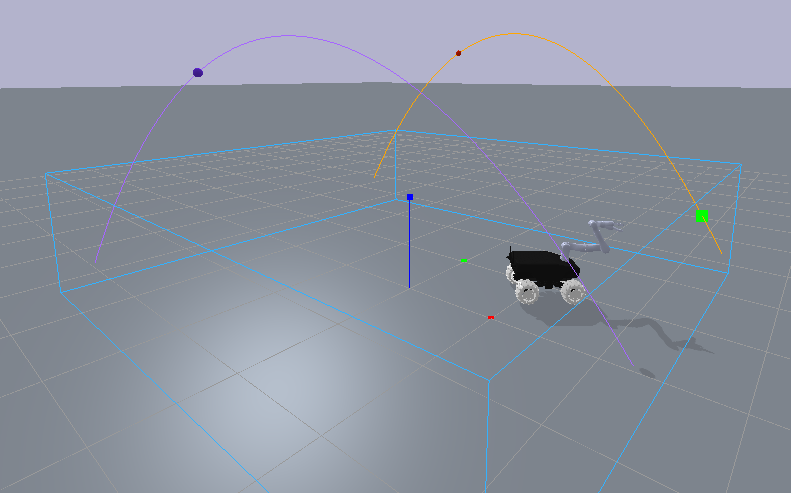
\includegraphics[width=\columnwidth]{image.png}
    \caption{Simulated single-ball catching task, showing the
    mobile robot, workspace boundaries and target interception point}
    \label{fig:image}
\end{figure}
\subsection{Expert and Demonstration Generation}
We extend the provided fixed-target expert with an interception planner that estimates the ball's velocity and acceleration from three position observations. It searches future points along the predicted path in $0.1\,\mathrm{s}$ increments, selecting the earliest feasible interception after re-entry into the workspace and a base position and heading from which the arm can reach it. Feasibility accounts for base travel, turning and arm movement, with extra time for settling. The existing base and arm controllers then move towards these planned goals, with replanning if the interception is missed by more than $1\,\mathrm{s}$. The model is trained to predict the wheel and arm commands produced by the expert.


\subsection{Dataset and Targeted Parking Perturbations}
Our training set contains 1,000 unique scenes, each recorded twice: once with the expert’s normal parking position and once with a shifted parking position, giving 2,000 demonstrations in total. The shifted demonstrations show how the robot can catch from imperfect base positions, following a similar principle to DART, which adds noise during expert demonstrations to teach recovery from errors~\cite{laskey2017}. We sample shifts along and perpendicular to the route from zero-mean Gaussians with standard deviations of $20$ and $50,\mathrm{mm}$, respectively, limiting the total shift to $150,\mathrm{mm}$.

Sampling these demonstrations every $0.02\,\mathrm{s}$ ($50\,\mathrm{Hz}$) gives 1,697,332 recorded training rows. Master seed 2026 generates the 1,000 training scene seeds and 200 separate evaluation scene seeds, with both demonstrations of each training scene kept in the training set. Evaluation scenes use the same generation rules and parameter distributions.



Demonstrations are resampled onto a $50\,\mathrm{Hz}$ grid, giving 1,697,332 rows in the recorded training dataset. Using master seed 2026, we generate 1,000 scene seeds for training and 200 separate seeds for evaluation, keeping both versions of each training scene in the training set. Evaluation scenes are generated using the same rules and parameter distributions as the training scenes.

\subsection{Observation Representation and Temporal Context}
% Raw observations, base-relative features, normalisation and history.
% Explain feature overlap and why history can help despite velocity inputs.
\subsection{Policy Architecture and Action Chunking}
% Ball encoder, pooling, robot trunk, dimensions and action semantics.
% One-ball pooling does not establish a multi-ball advantage.
% State prediction horizon, execution horizon, query-relative joint
% references and fixed low-level servos separately from learned inference.
\subsection{Training Configuration}
% Loss, optimiser, training steps, batch size, seeds and parameter count.
% Table I slot: selected 50 Hz configuration and relevant predecessor.

\section{Evaluation Protocol}
% Approx. 0.5 page. Explain why each metric measures a project requirement.
\subsection{Closed-Loop Episodes and Capture Conditions}
% Define valid capture window, strict radius threshold and termination.
% Closest approach is not physical grasping. Include every scored episode.
% The reused 200-scene benchmark is not an untouched final test set.
\subsection{Accuracy and Statistical Uncertainty}
% Define per-scene minimum distance and catch-rate equations here.
% Mean, median, tail quantiles, maximum and success-radius ECDF.
% Separate paired scene uncertainty from training-seed variation.
% Do not invent historical per-scene curves or multi-seed uncertainty.
\subsection{Diagnostic and Reproducibility Checks}
% Along/cross/vertical components and phase-aligned ML rollout traces.
% Define the correction coefficient from code before using it.
% Expert references are offline annotations, not runtime takeovers.
% Freeze data/config/weights and check Torch/NumPy export agreement.

\section{Results and Failure Analysis}
% Approx. 2 pages. Organise by hypotheses rather than experiment chronology.
\subsection{Accuracy and Development Comparisons}
% Table II slot: baseline -> relative features -> offset data -> encoder
% -> 50 Hz timing. Label single-seed versus multi-seed rows explicitly.
% Describe dataset-size, architecture and timing confounds.
% Figure 2 slot: radius curve and tail distribution from available episodes.
\subsection{Parking Error and Base--Arm Compensation}
% Finding A from report_angles.md, qualified against the actual evidence.
% Figure 3 candidate: along/cross-track parking versus hand error.
% Check the correction-coefficient definition and numbers in source code.
% Include DART/DAgger only if the implementation and comparison are audited.
\subsection{Stopping Behaviour and the Command-Hold Hypothesis}
% Finding B: distinguish expert-state residuals, stop-transition error,
% and learner-state drift. Keep 25 Hz and 50 Hz evidence separate.
% Figure 3 alternative: braking commands and realised motion near stopping.
% A centred residual does not establish that the model is always correct.
\subsubsection{Available diagnostic evidence}
% Populate only after verifying the relevant logged tests and their scope.
\subsubsection{Unverified replay and interpolation findings}
% BLANK: no replay confirmation or interpolation benefit is assumed.
% Do not run or score non-ML controller interventions as policy successes.
\subsection{Negative Results from Broader Parking Perturbations}
% Finding C: matched-offset variants, prespecified bar if documented,
% actual outcomes and limits of the inference about data coverage.
\subsection{Robustness, Generalisation and Efficiency}
% Compact table slot: parameters, dataset size, training and inference time.
% Distinguish same-distribution held-out scenes from distribution shift.
\subsubsection{Observation noise and actuation latency}
% BLANK: insert completed frozen-policy robustness results if available.
\subsubsection{Out-of-distribution trajectories}
% BLANK: insert completed OOD evaluation if available.
\subsubsection{Computational cost}
% Fill verified costs; leave unmeasured CPU latency blank.
\subsection{Historical Result and Local Reproduction}
% Separate recorded 24.74 mm historical mean from 52.37 mm local mean.
% Report full aggregates and rare large misses; never substitute a trimmed
% mean. Dataset/platform differences are observations, not proven causes.
% Historical original weights and raw distributions remain unavailable.

\section{Discussion and Limitations}
% Approx. 0.75 page; reduce elsewhere if figures need more room.
\subsection{What the Evidence Supports}
% Connect representation, targeted coverage and timing to measured results.
% Explain the project-specific evaluation contribution without claiming
% standard ECDFs or offset augmentation are globally novel.
\subsection{Limits of the Braking Explanation}
% State what would discriminate command holding from other explanations.
% Include counterexamples; do not turn a plausible mechanism into a finding.
\subsection{Validity, Reproducibility and Remaining Gaps}
% Confounded comparisons, reused scenes, single-seed final timing result,
% platform mismatch, ideal state inputs, no hardware or grasp validation.
% Missing robustness/OOD results remain explicit gaps.
\subsection{Future Work}
% Suggested tests only: frozen independent evaluation, seed replication,
% perception robustness and further stopping diagnosis. No promised gains.

\section{Conclusion}
% Approx. 0.25 page. Answer the research question using verified evidence.
% State achieved scope and limits; no claim of 80% catches below 10 mm.

% Approx. 0.5 page reserved for verified primary references.
% Add citations during the writing pass; do not fabricate bibliography data.
\begin{thebibliography}{00}
% BLANK: behaviour cloning, DeepSets, simulator/kinematics and reused code.
\end{thebibliography}

% Separate statement, up to one additional page under the assignment brief.
% Keep outside the six-page technical-report budget.
\clearpage
\section*{Contribution Statement}
% BLANK: group members must supply their actual contributions.

\end{document}
